\chapter{User Study Design}\label{chapter:study-design}

\section{Introduction}\label{sec:study-design-intro}
This chapter presents the design and methodology of a user study conducted to investigate the third research question: \emph{How does the implemented AR system influence collaboration dynamics, user satisfaction and performance during industrial task execution, particularly in relation to different task variants and different types of users (e.g., varying personality traits)?} Building upon the technical implementation described in the previous chapter, this empirical investigation provides insights into the practical effectiveness of AR-supported collaborative work in industrial settings through systematic evaluation of user interactions, performance metrics, and subjective experiences across different experimental conditions.

Figure~\ref{fig:user-study-procedure} provides an overview of the complete study procedure, illustrating the structured sequence from participant introduction and familiarisation through task execution and data collection phases.

\begin{figure}[!htb]
    \centering
    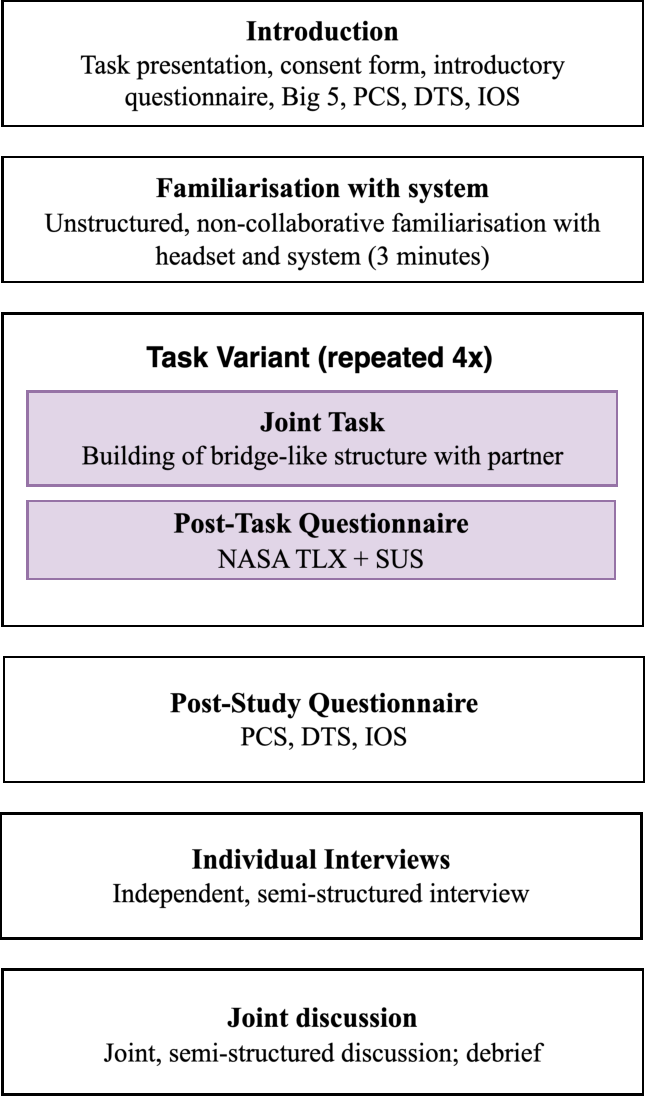
\includegraphics[width=0.4\textwidth]{assets/05/user-study-procedure.pdf}
    \caption{Overview of the user study procedure}
    \label{fig:user-study-procedure}
\end{figure}

\subsection{Organisational overview}\label{subsec:organisational-overview}
The study was conducted in March 2025 in a classroom setting at the Institute of Manufacturing, University of Cambridge. The experimental setup and data collection underwent the approval process of the Department of Engineering of the University of Cambridge. Prior to the experiment, participants received a detailed explanation of the study, its objectives, the specific data that would be collected as well as their right to withdraw from the study at any time and have their data deleted without consequences. For their participation, they received a compensation in the form of a 10 GBP Amazon.com gift card, supplied by the University of Cambridge.

\subsection{Participant Characteristics}\label{subsec:participant-characteristics}
The participants were a convenience sample of 16 STEM students currently enrolled at or visiting the University of Cambridge. Further details about the participant population are provided in Chapter~\ref{chapter:results}.
The participants were randomly split into 8 pairs of participants. The cohort's tight alignment prioritised population validity (i.e. fidelity to the real-world operator base of industrial AR systems) over external validity to a more general audience.


\section{Experimental Design}\label{sec:experimental-design}
\subsection{Task Design}\label{subsec:task-design}
The study employs a simplified bridge construction task inspired by civil engineering education contexts, specifically drawing from the bridge building component of the \emph{Design and Construction 2} course that is a mandatory part of the civil engineering curriculum at the Technical University of Munich\footnote{\url{https://www.cee.ed.tum.de/en/hbb/teaching/civil-engineering-bsc-msc/building-construction-ii-1/}}\footnote{\url{https://www.youtube.com/watch?v=XPyD-n9JS3Y}}. This task design provides several advantages for studying collaboration dynamics while maintaining relevance to industrial work.

The bridge construction task offers measurable, quantitative outcomes (task completion time, bridge load capacity) while requiring genuine coordination between participants. Unlike purely creative or planning tasks, the construction work involves physical manipulation of objects, creating opportunities to study how AR mediates spatial awareness and joint action coordination in industrial contexts.

The educational inspiration of the task ensures accessibility without requiring deep prior domain knowledge, allowing the study to isolate collaboration factors rather than confounding them with expertise differences. The nature of the construction task maintains the essential characteristics of industrial assembly work: sequential dependencies, spatial coordination requirements, and quality constraints, while reducing complexity that might obscure collaboration dynamics.

This approach maintains ecological validity as outlined by \cite{personeni2023ecological}, who emphasises that tasks retain ecological viability when task, environment, and user roles approximate their real-world counterparts. In our implementation, the bridge construction task conducted by engineering students in a classroom setting closely mirrors this framework, with the virtual bridge assembly task being a close approximation of the real-world bridge construction task, the classroom environment carrying over almost directly, and participants being sampled from a population of engineering students.

\subsection{Gameplay Mechanics}\label{subsec:gameplay-mechanics}
The core gameplay loop centres on connecting two starting blocks positioned 2m apart (based on their centre points) in the virtual workspace. Participants must collaborate to build a bridge structure that spans this gap using a variety of virtual building blocks with different costs and shapes.

\subsubsection{Building Block System}
The system provides participants with access to seven different types of building blocks, each with distinct costs and structural properties. Figure~\ref{fig:shapes-pricing-grid} shows the complete inventory of available blocks with their associated pricing structure. Participants could spawn unlimited blocks throughout the task, with real-time cost tracking displayed through a small UI element tracked by their hand for continuous visibility without obstructing the main workspace.

The grid texture visible in the images indicates scale, with each grid square representing 10cm x 10cm. For example, the small cube measures 10cm x 10cm x 10cm, while the big cube is composed of four small cubes arranged in a 2x2x2 configuration, resulting in dimensions of 20cm x 20cm x 20cm. Other block types maintain proportional scaling relative to these base dimensions.

\begin{figure}[htbp]
    \centering
    \begin{subfigure}[b]{0.28\textwidth}
        \centering
        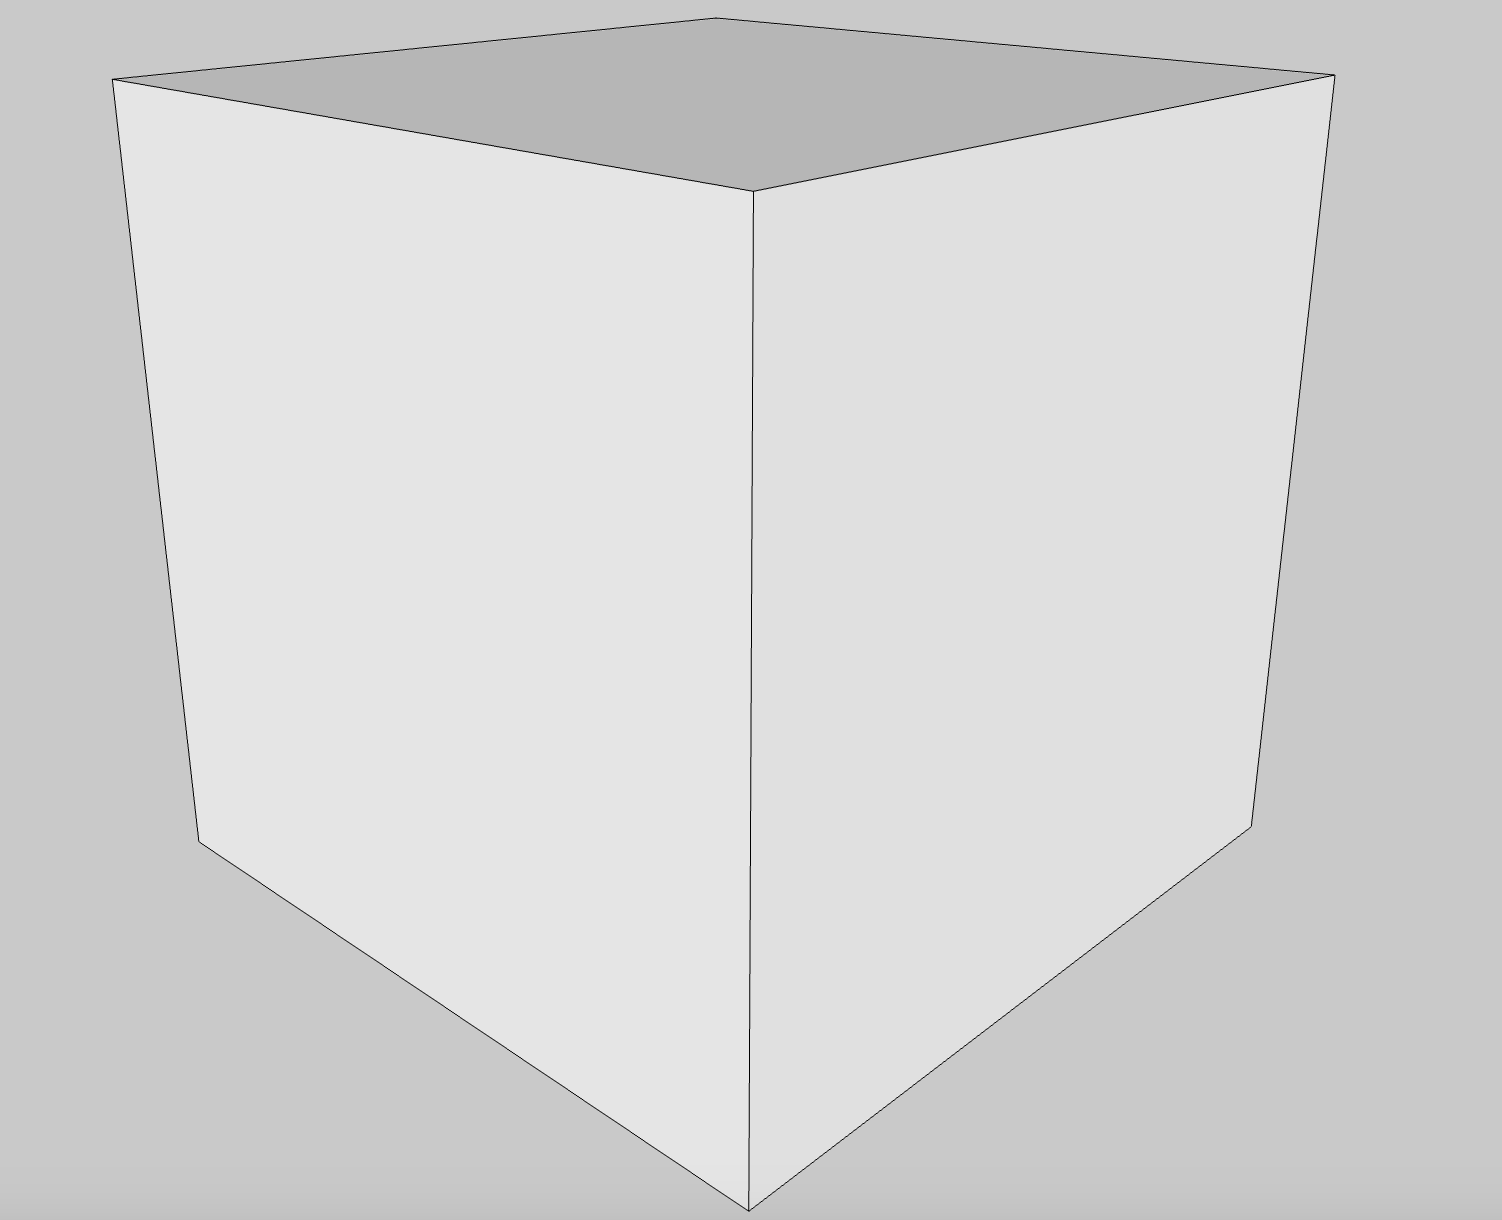
\includegraphics[width=0.75\textwidth]{user-study-analysis/meta/shapes/cube.png}
        \caption{Small Cube\\Cost: 1}
        \label{fig:small-cube}
    \end{subfigure}
    \hfill
    \begin{subfigure}[b]{0.28\textwidth}
        \centering
        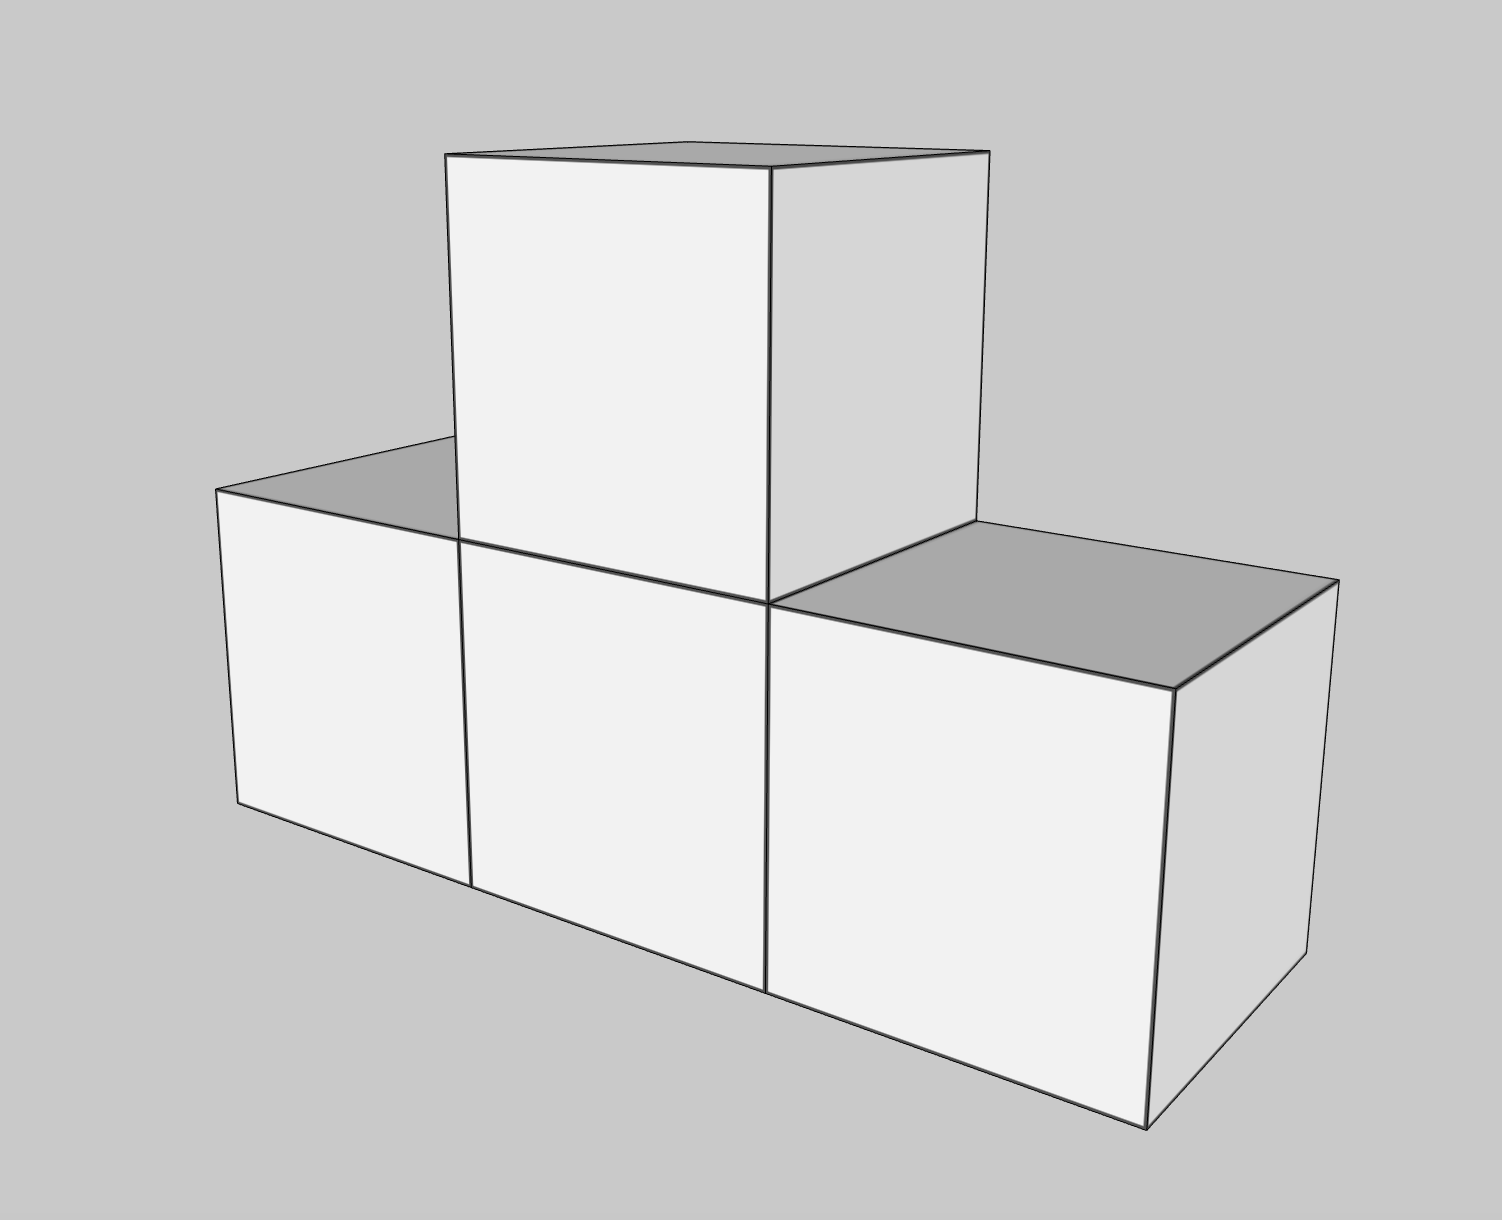
\includegraphics[width=0.75\textwidth]{user-study-analysis/meta/shapes/t-shape.png}
        \caption{T-Shape\\Cost: 2}
        \label{fig:t-shape}
    \end{subfigure}
    \hfill
    \begin{subfigure}[b]{0.28\textwidth}
        \centering
        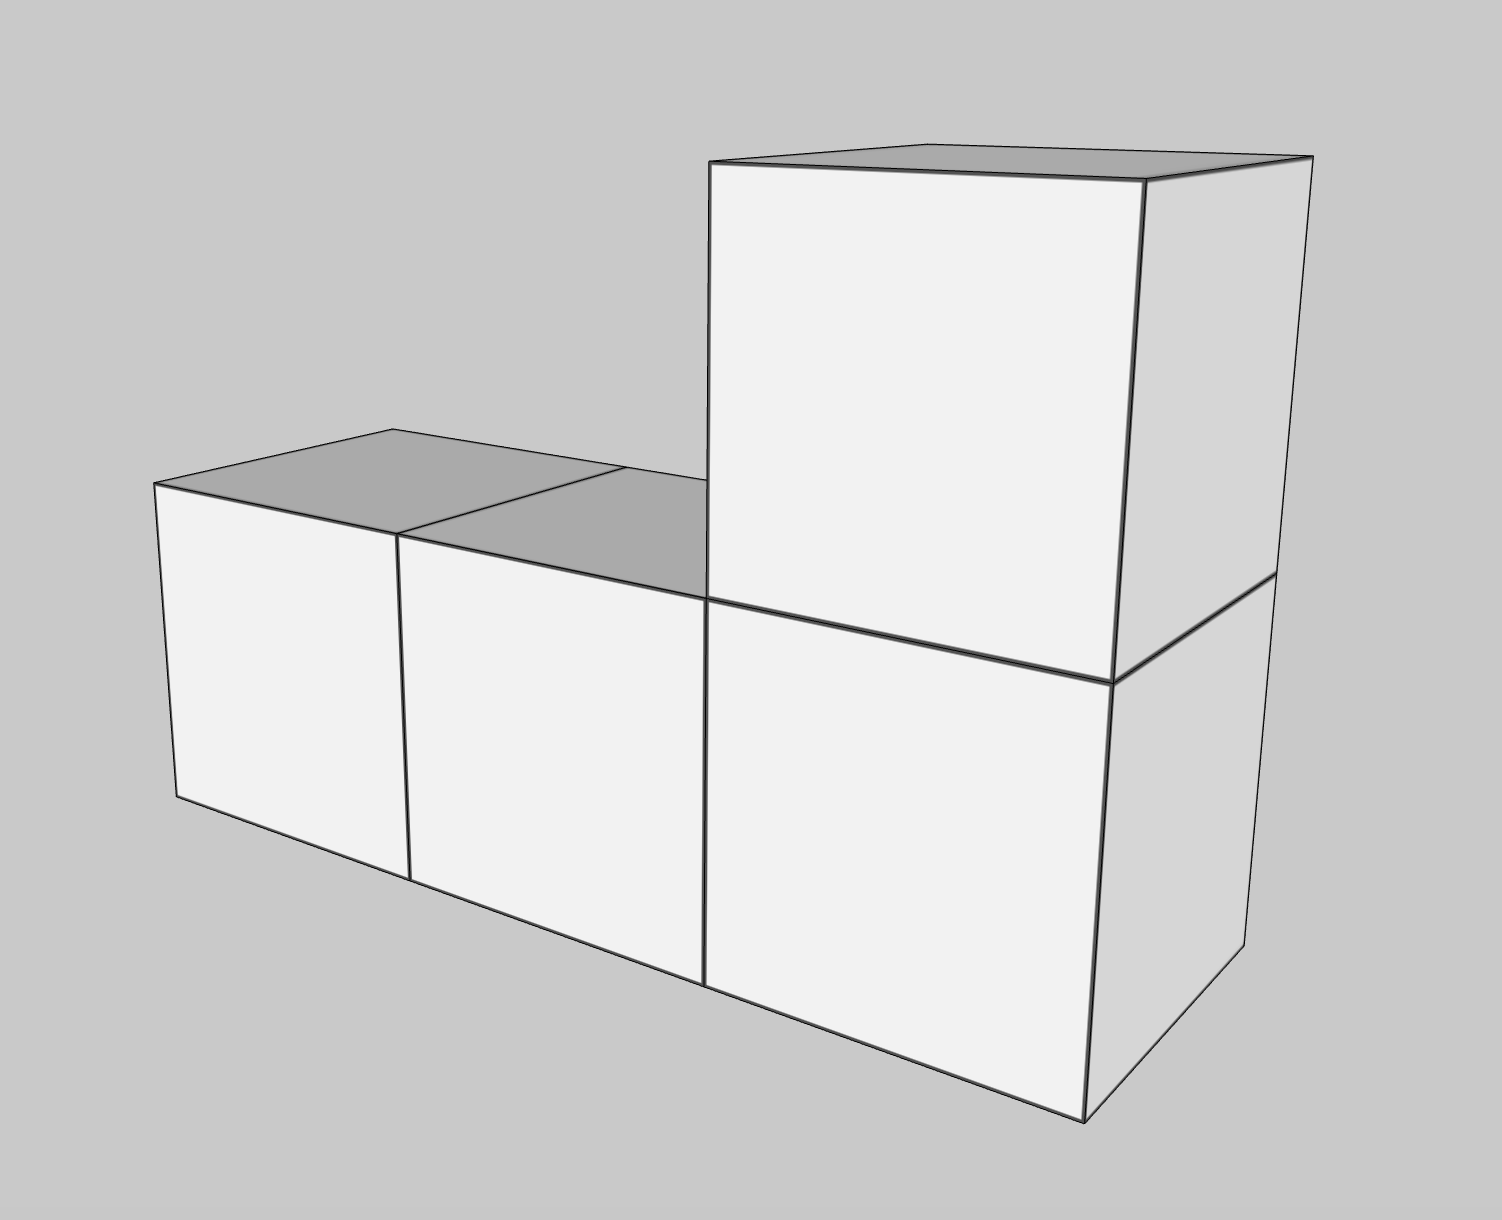
\includegraphics[width=0.75\textwidth]{user-study-analysis/meta/shapes/l-shape.png}
        \caption{L-Shape\\Cost: 2}
        \label{fig:l-shape}
    \end{subfigure}
    
    \vspace{0.5cm}
    
    \begin{subfigure}[b]{0.28\textwidth}
        \centering
        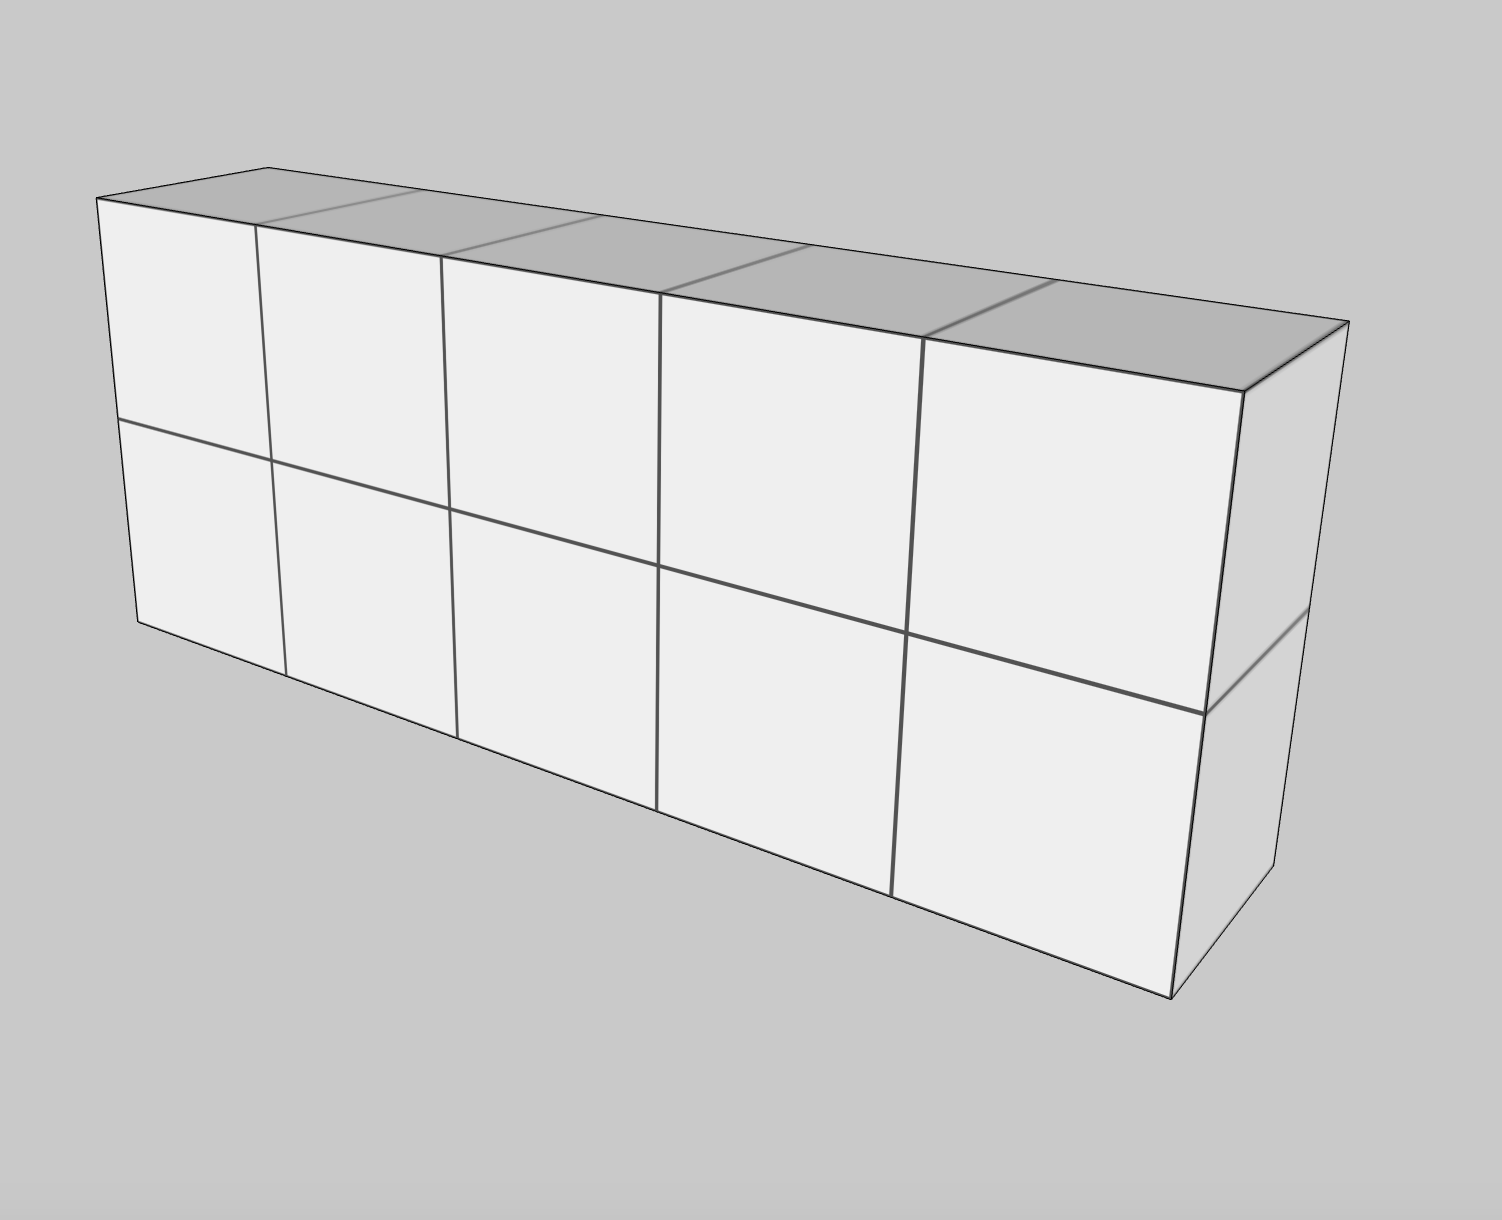
\includegraphics[width=0.75\textwidth]{user-study-analysis/meta/shapes/plank.png}
        \caption{Plank\\Cost: 10}
        \label{fig:plank}
    \end{subfigure}
    \hfill
    \begin{subfigure}[b]{0.28\textwidth}
        \centering
        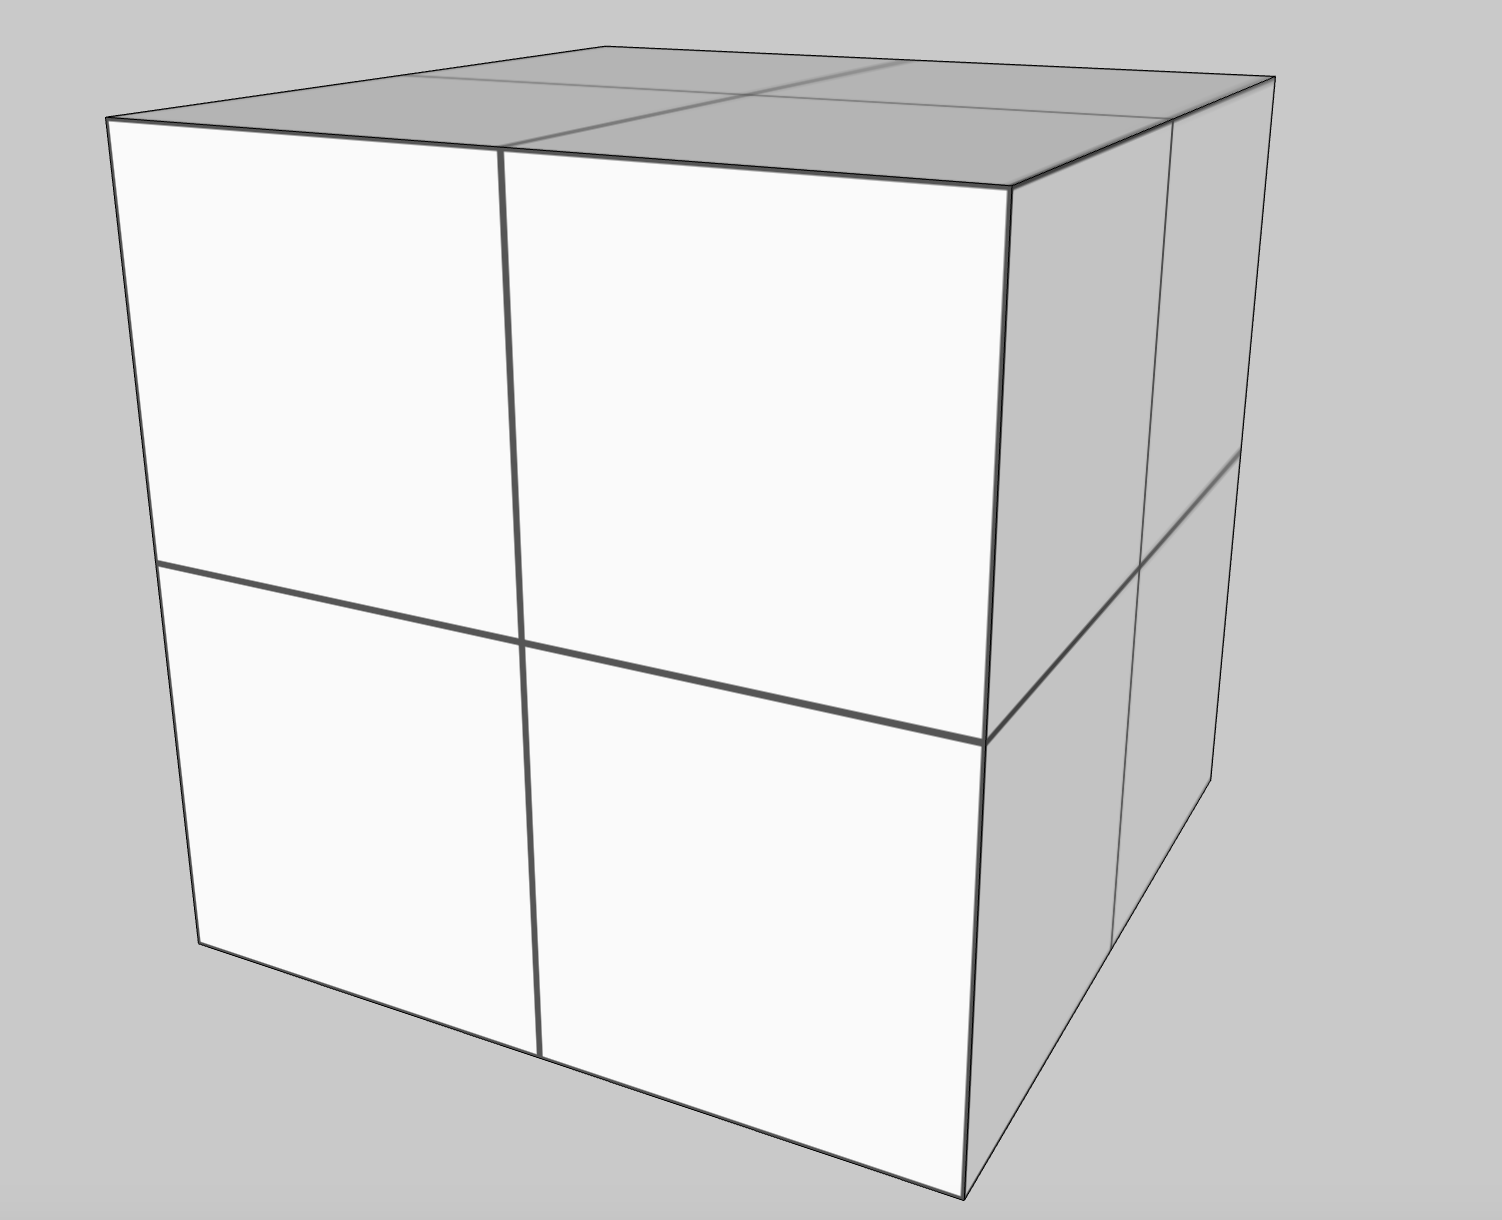
\includegraphics[width=0.75\textwidth]{user-study-analysis/meta/shapes/big-cube.png}
        \caption{Big Cube\\Cost: 8}
        \label{fig:big-cube}
    \end{subfigure}
    \hfill
    \begin{subfigure}[b]{0.28\textwidth}
        \centering
        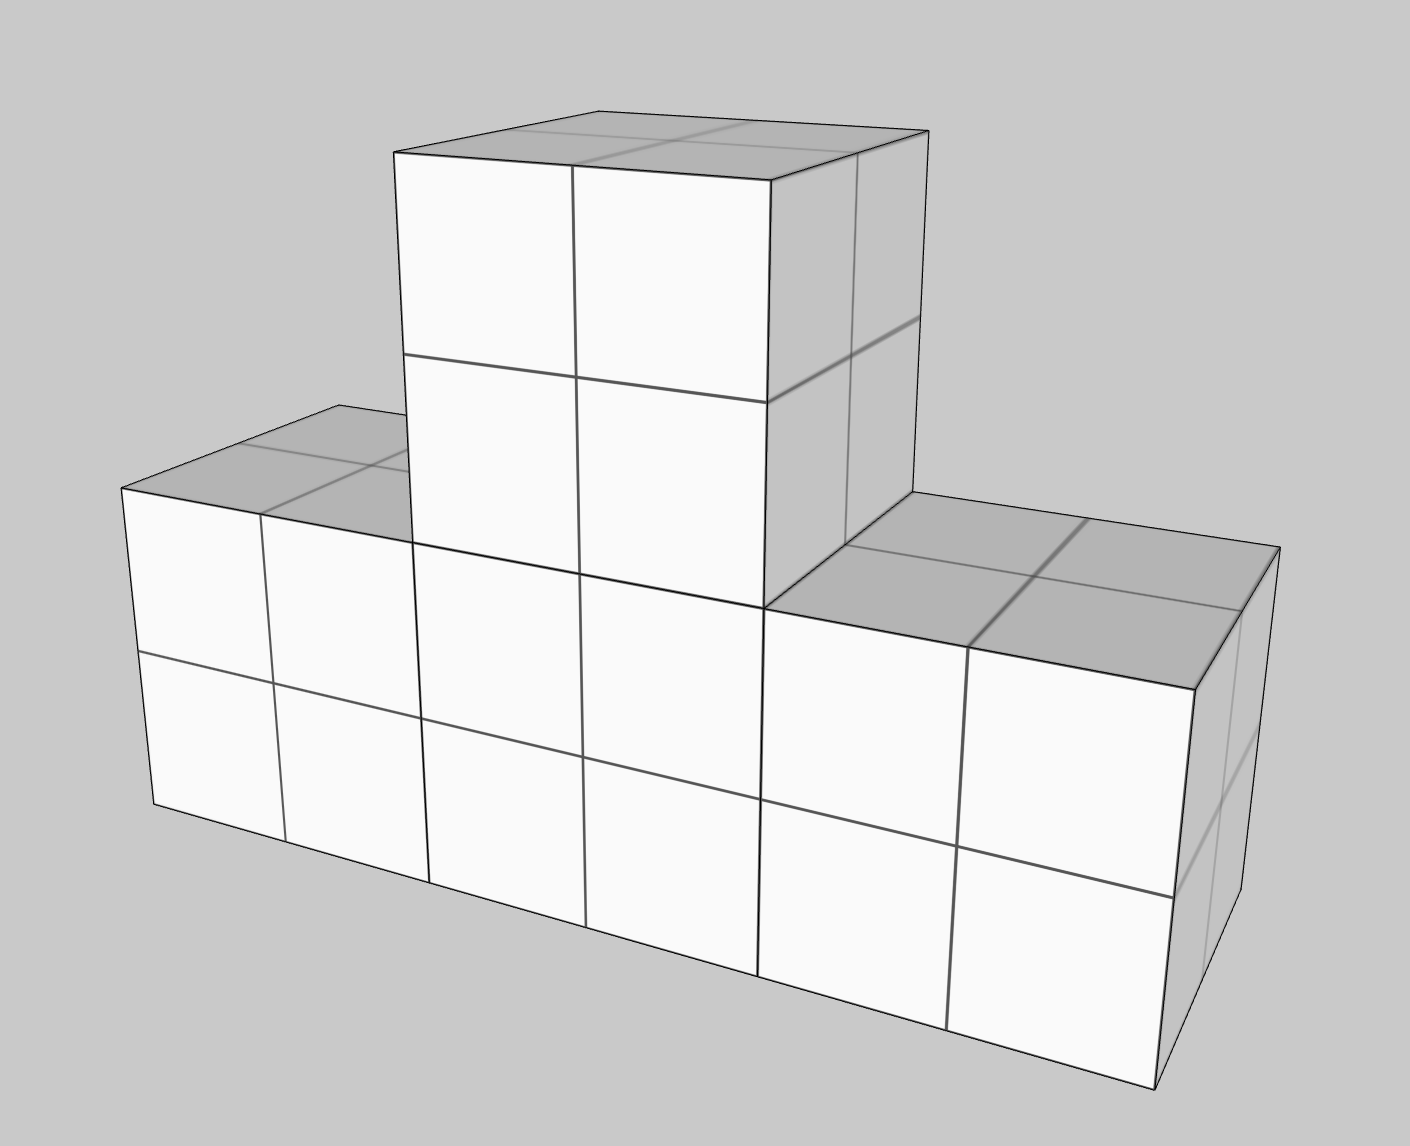
\includegraphics[width=0.75\textwidth]{user-study-analysis/meta/shapes/big-t-shape.png}
        \caption{Big T-Shape\\Cost: 50}
        \label{fig:big-t-shape}
    \end{subfigure}
    
    \vspace{0.5cm}
    
    \begin{subfigure}[b]{0.28\textwidth}
        \centering
        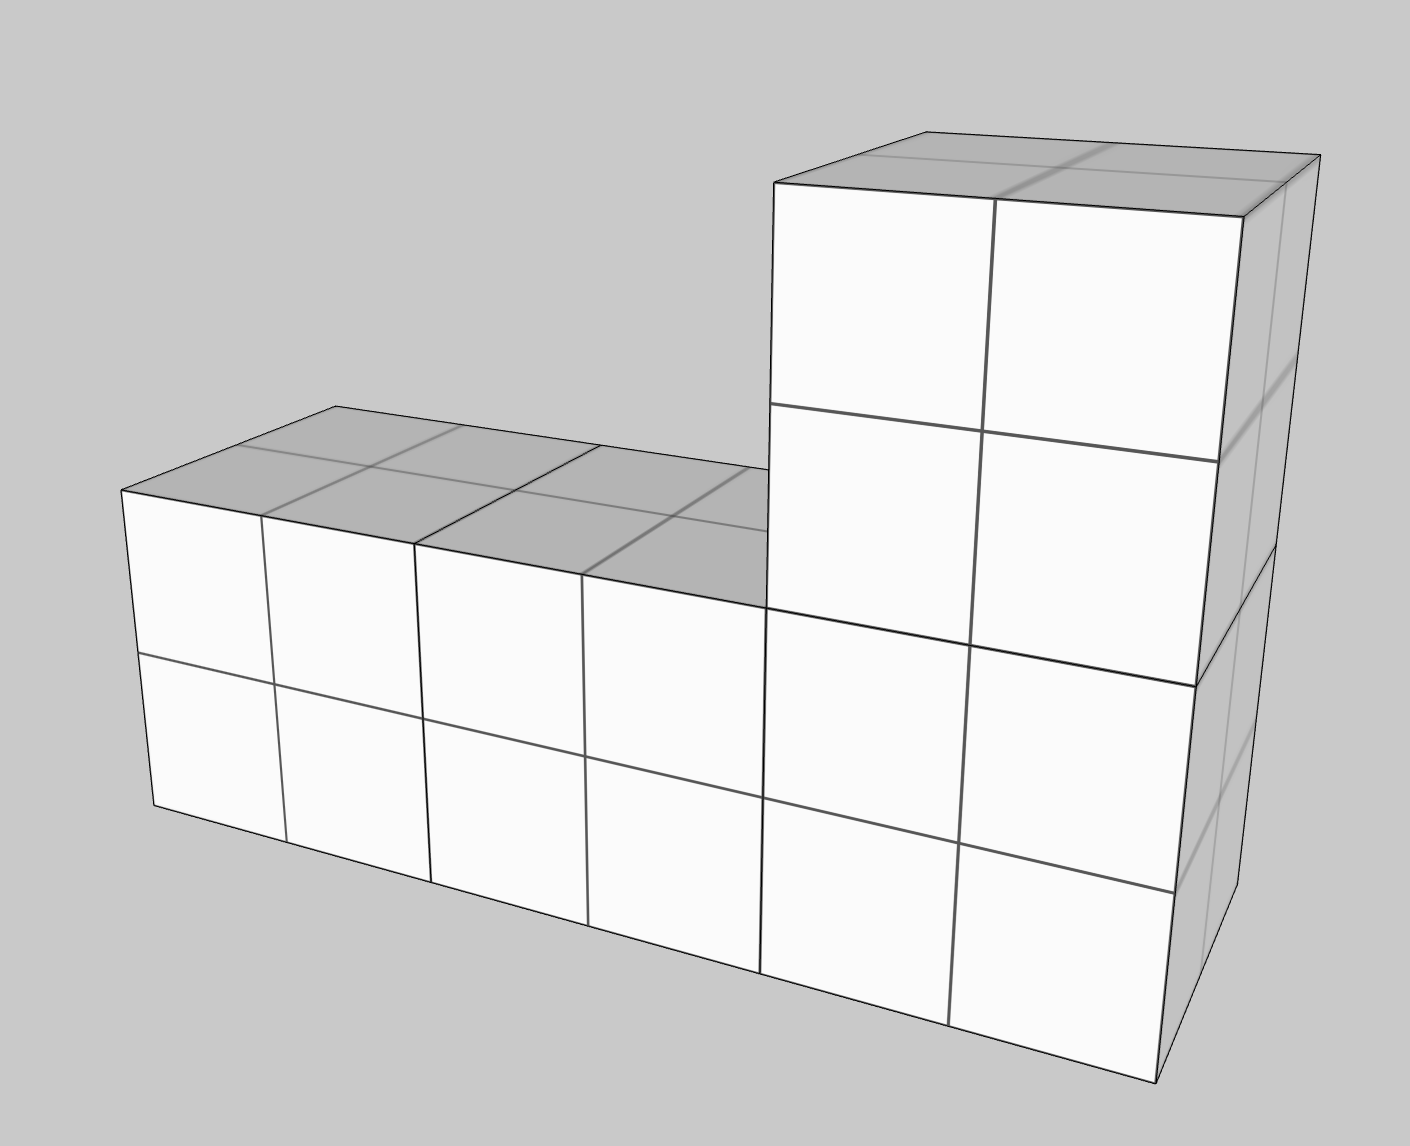
\includegraphics[width=0.75\textwidth]{user-study-analysis/meta/shapes/big-l-shape.png}
        \caption{Big L-Shape\\Cost: 50}
        \label{fig:big-l-shape}
    \end{subfigure}
    
    \caption{Grid of available building blocks with their associated costs.}
    \label{fig:shapes-pricing-grid}
\end{figure}

\subsubsection{Environmental Variants}
In addition to the four task variants described in Section~\ref{subsec:study-design-overview}, the system included four distinct environmental configurations to provide inter-task variability and try to prevent participants from developing overly systematic approaches. These environments featured transparent red blocker zones positioned strategically within the workspace. Any blocks placed within these zones would despawn after a brief grace period, forcing participants to build around these obstacles rather than constructing direct linear spans.

As detailed in Chapter~\ref{chapter:artifact-implementation}, these deletion zones serve three purposes: they introduce spatial constraints that require creative problem-solving, they provide task variability that maintains engagement across multiple rounds, they prevent the development of rote solutions, and they pragmatically allow participants to remove accidentally spawned or no longer needed blocks.

Figure~\ref{fig:environment-variants} illustrates the four environmental configurations used in the study, each presenting different spatial challenges and collaborative coordination requirements.

\begin{figure}[htbp]
    \centering
    \begin{subfigure}[b]{0.48\textwidth}
        \centering
        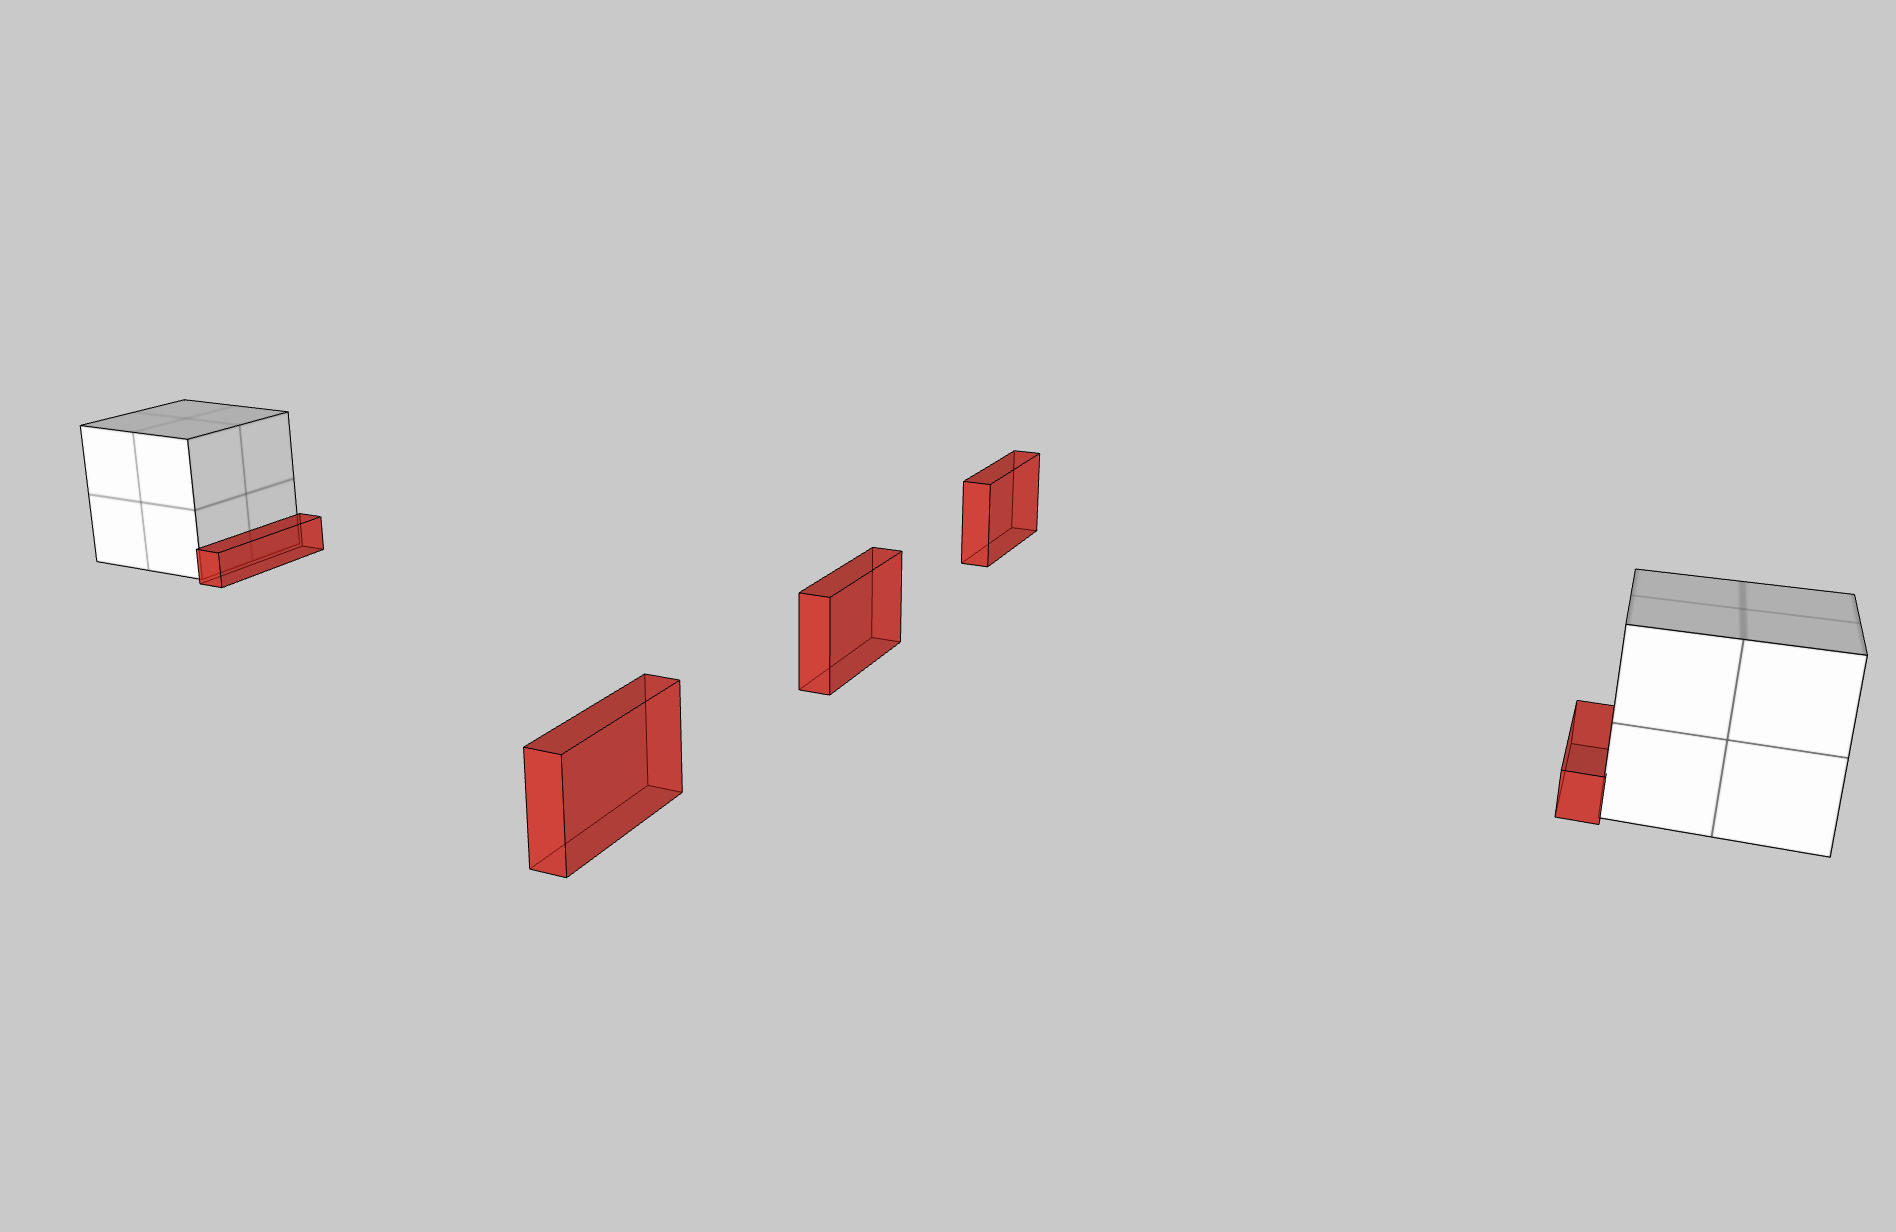
\includegraphics[width=\textwidth]{assets/05/environment-0.png}
        \caption{Environment 0}
        \label{fig:env-0}
    \end{subfigure}
    \hfill
    \begin{subfigure}[b]{0.48\textwidth}
        \centering
        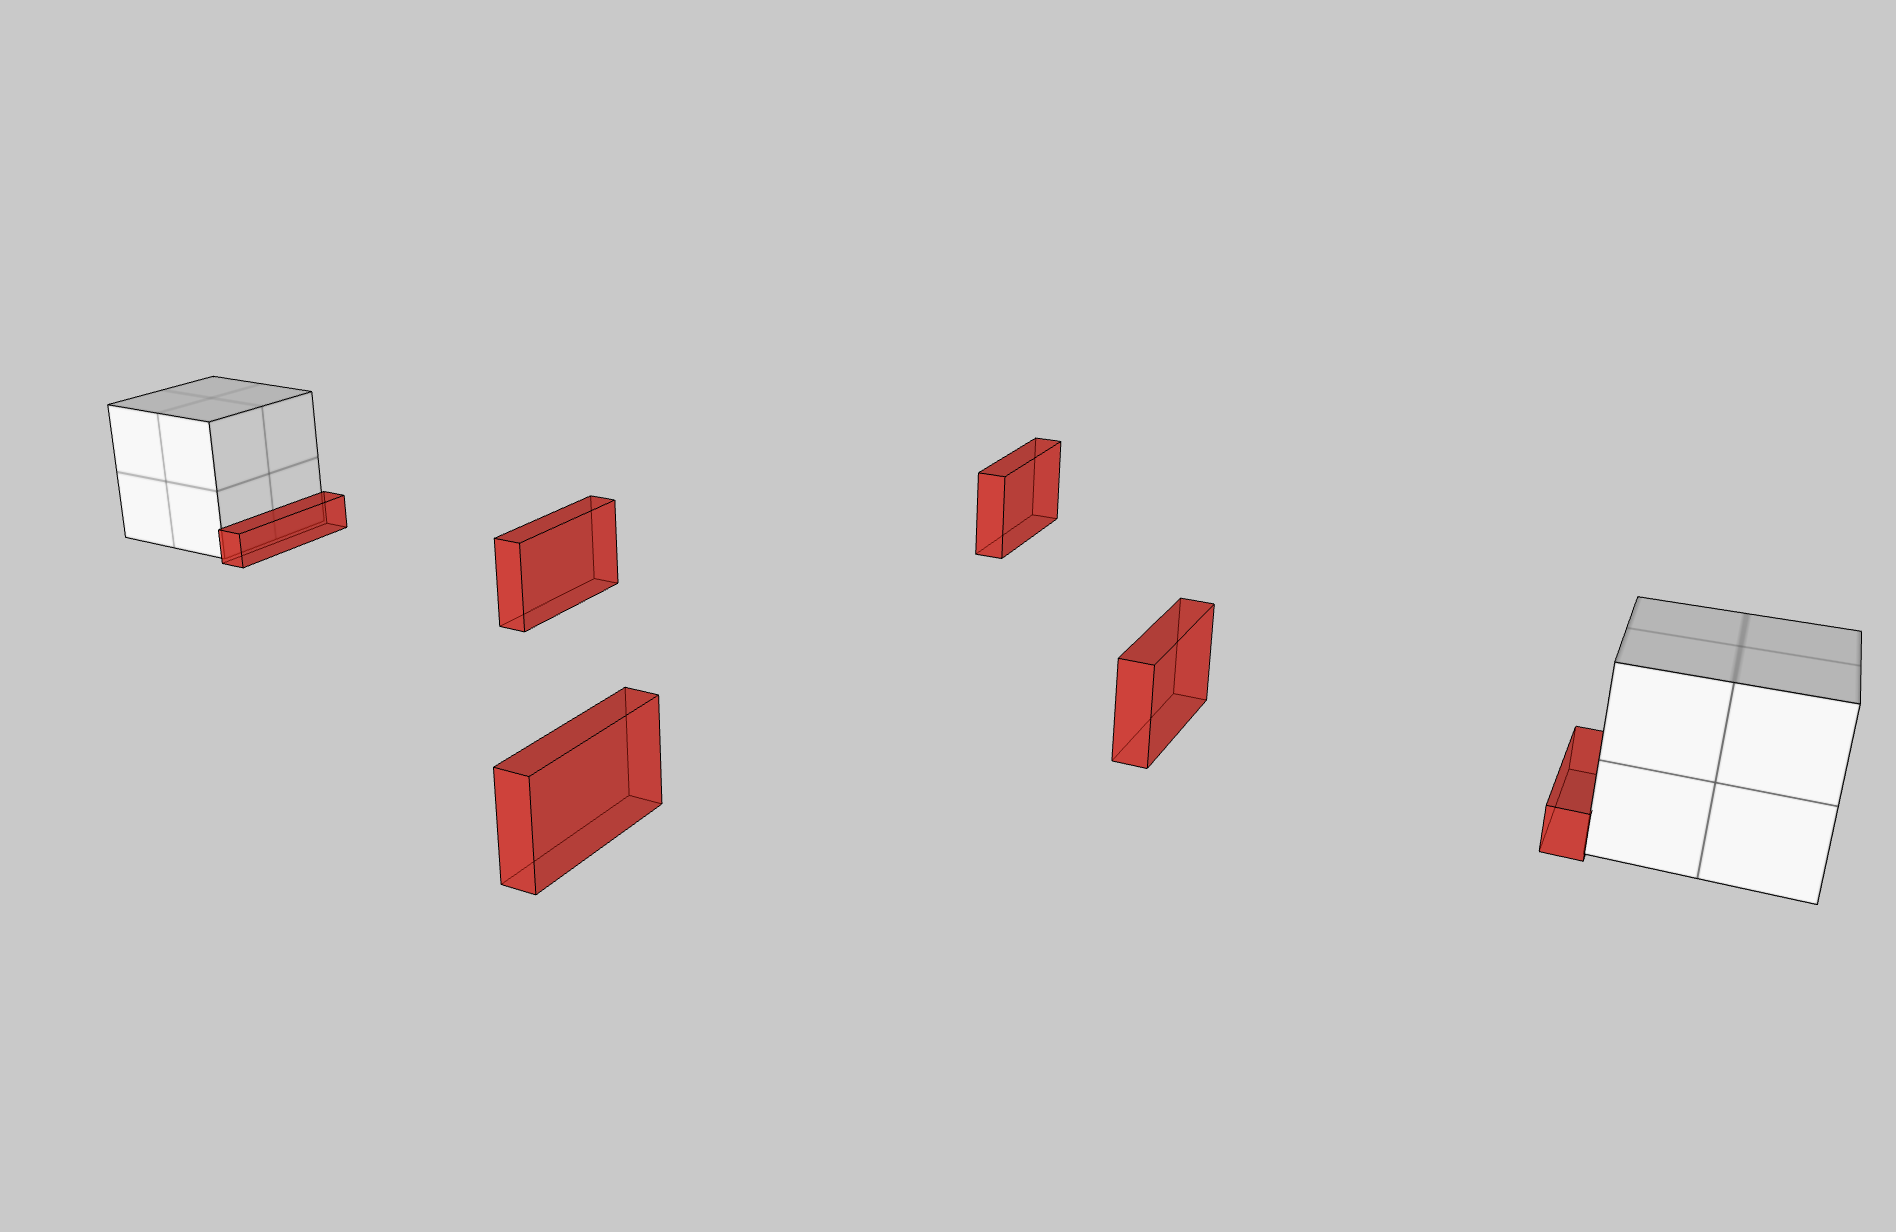
\includegraphics[width=\textwidth]{assets/05/environment-1.png}
        \caption{Environment 1}
        \label{fig:env-1}
    \end{subfigure}
    
    \vspace{0.5cm}
    
    \begin{subfigure}[b]{0.48\textwidth}
        \centering
        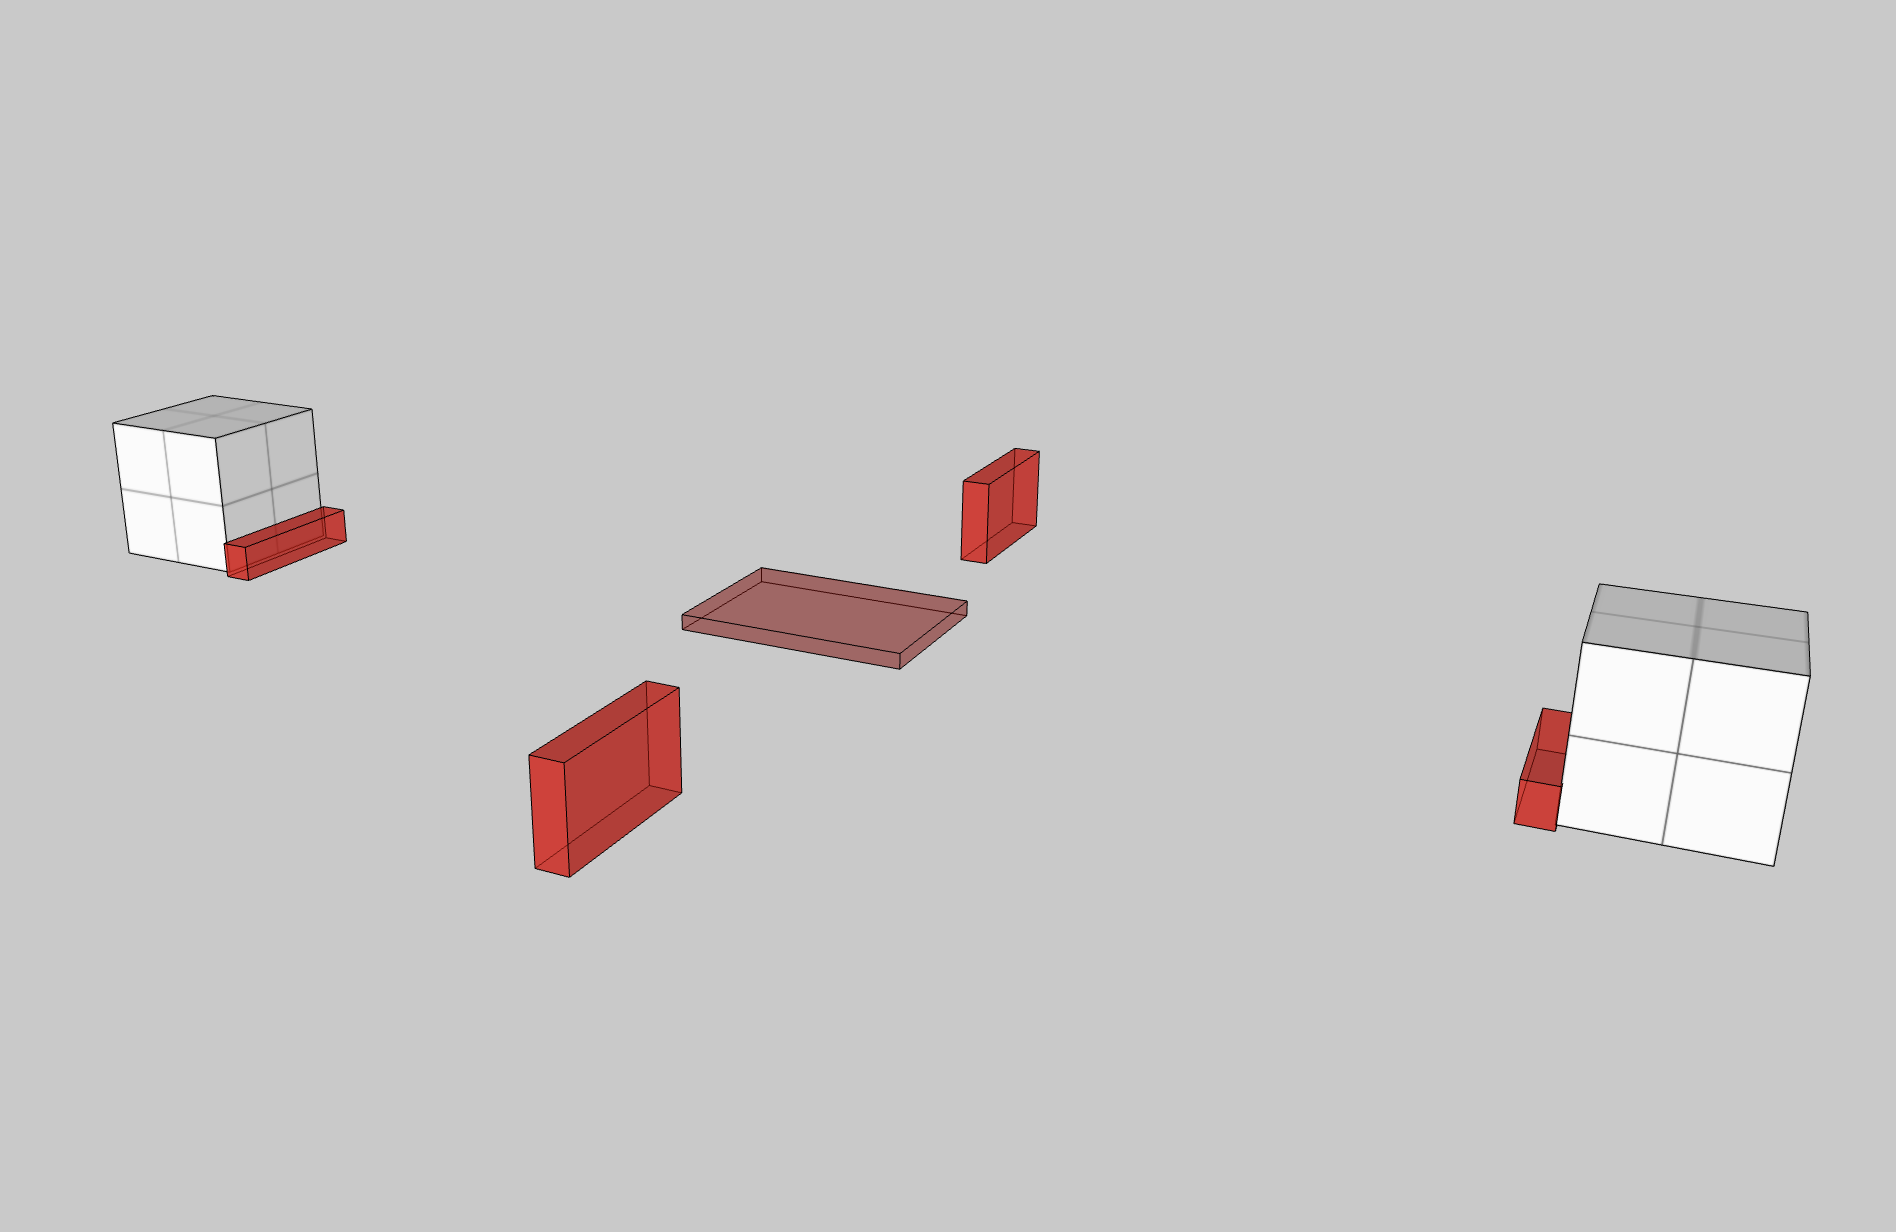
\includegraphics[width=\textwidth]{assets/05/environment-2.png}
        \caption{Environment 2}
        \label{fig:env-2}
    \end{subfigure}
    \hfill
    \begin{subfigure}[b]{0.48\textwidth}
        \centering
        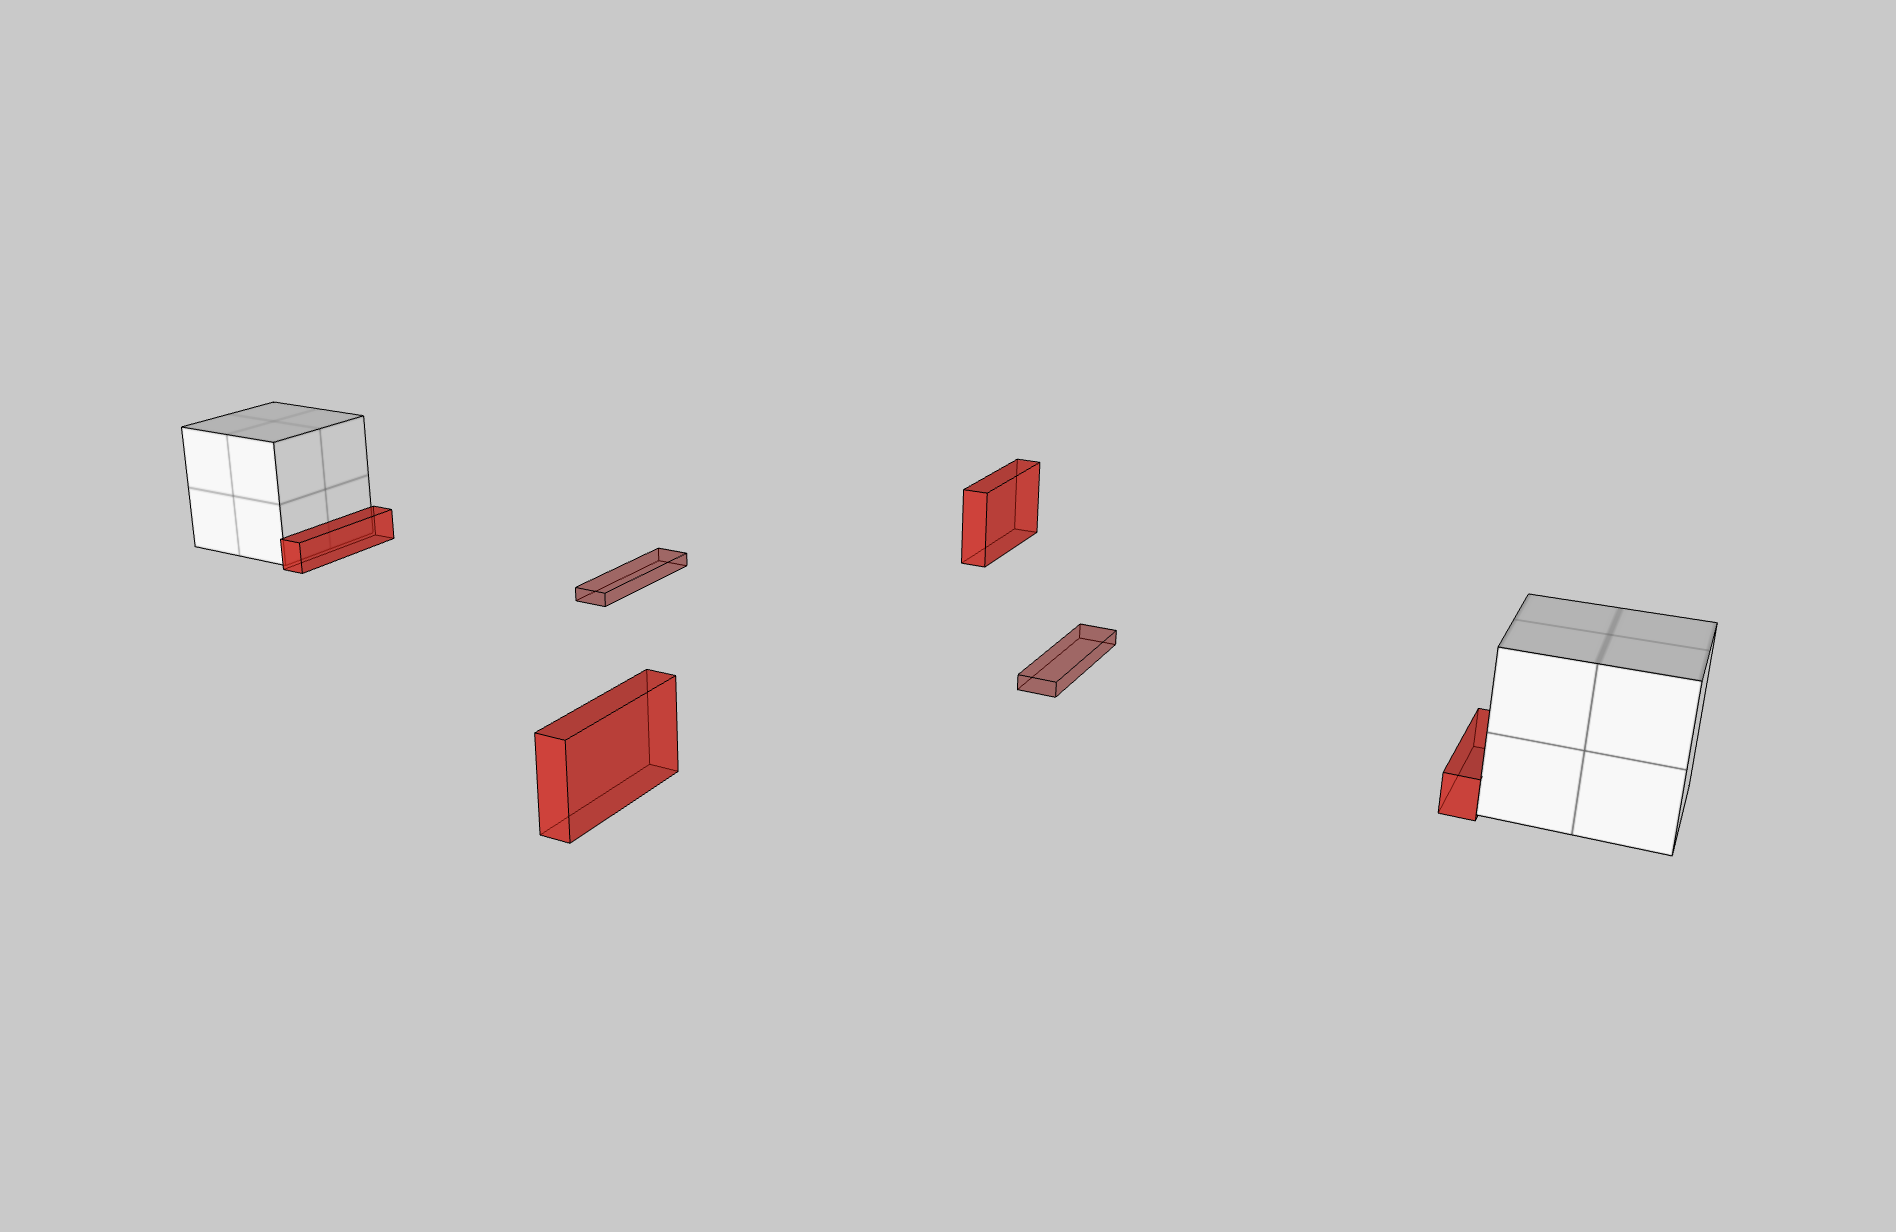
\includegraphics[width=\textwidth]{assets/05/environment-3.png}
        \caption{Environment 3}
        \label{fig:env-3}
    \end{subfigure}
    \caption{The four environmental variants used in the study, showing different configurations of transparent red blocker zones that required participants to build around spatial obstacles.}
    \label{fig:environment-variants}
\end{figure}

\subsubsection{Environmental Randomisation}
The environmental configurations were randomised using a 4-treatment Williams Latin square to control for order effects\cite{williams1949experimental}. Table~\ref{tab:environment-randomisation} shows the environmental randomisation scheme across participant pairs.

\begin{table}[htbp]
    \centering
    \begin{tabular}{c|cccc}
        \textbf{Pair} & \textbf{Period 1} & \textbf{Period 2} & \textbf{Period 3} & \textbf{Period 4} \\
        \hline
        1 & Env 0 & Env 1 & Env 3 & Env 2 \\
        2 & Env 1 & Env 3 & Env 2 & Env 0 \\
        3 & Env 3 & Env 2 & Env 0 & Env 1 \\
        4 & Env 2 & Env 0 & Env 1 & Env 3 \\
        5 & Env 1 & Env 3 & Env 2 & Env 0 \\
        6 & Env 3 & Env 2 & Env 0 & Env 1 \\
        7 & Env 2 & Env 0 & Env 1 & Env 3 \\
        8 & Env 0 & Env 1 & Env 3 & Env 2 \\
    \end{tabular}
    \caption{Environmental configuration randomisation scheme across participant pairs, randomised using a 4-treatment Williams Latin square, replicated twice\cite{williams1949experimental}}
    \label{tab:environment-randomisation}
\end{table}

\subsection{Study Design Overview}\label{subsec:study-design-overview}
The study design is a within-subjects design, with participants completing all conditions. The four conditions were:
\begin{itemize}
    \item \textbf{Normal}: Participants are simply told to assemble a bridge.
    \item \textbf{Shop-floor environment}: Participants are told to assemble a bridge, but are not allowed to speak (simulating a loud shop-floor environment).
    \item \textbf{Time limited}: Participants are told to assemble a bridge, but once they spawn the first block, they have a maximum of five minutes to complete the task.
    \item \textbf{Split objectives}: Participants are told to optimise for different outcomes (one participant is told to optimise for the bridge being strong, the other for the bridge being cheap) to simulate a real-world scenario where different participants have different priorities.
\end{itemize}
The condition order was randomised using a twice-replicated Williams-type balanced Latin square to prevent order effects\cite{williams1949experimental}. The resulting sequence assignments are shown in Table~\ref{tab:latin-square}.

\begin{table}[ht]
    \centering
    \begin{tabular}{c|cccc}
      Sequence & Period 1    & Period 2    & Period 3      & Period 4      \\
      \hline
      1        & Open Ended  & Timed       & Silent        & Roleplay      \\
      2        & Timed       & Roleplay    & Open Ended    & Silent        \\
      3        & Silent      & Open Ended  & Roleplay      & Timed         \\
      4        & Roleplay    & Silent      & Timed         & Open Ended    \\
      5        & Open Ended  & Timed       & Silent        & Roleplay      \\
      6        & Timed       & Roleplay    & Open Ended    & Silent        \\
      7        & Silent      & Open Ended  & Roleplay      & Timed         \\
      8        & Roleplay    & Silent      & Timed         & Open Ended    \\
    \end{tabular}
    \caption{Task variant randomisation scheme across participant pairs, randomised using a 4-treatment Williams Latin square, replicated twice\cite{williams1949experimental}}
    \label{tab:latin-square}
\end{table}

\subsection{Instructions}\label{subsec:task-instructions}
To ensure participants had an equal understanding of the task, they were given the following instructions verbatim:

\begin{itemize}
    \item Treat the task as a bridge building task, where the goal is to assemble a bridge that connects the two base points. Any structure that connects the two base points will be accepted.
    \item Any objects placed in the red areas will be deleted after a few seconds.
    \item Treat this as a civil engineering task, meaning you should optimise three goals:
    \begin{itemize}
        \item Strength: Make the bridge as stable as possible.
        \item Cost: Do so using the cheapest parts possible.
        \item Time: Finish the task as fast as possible.
    \end{itemize}
\end{itemize}
Participants were also given up to 3 minutes to familiarise themselves with the Hololens headset, the user interface and the building mechanics before the first task variant was presented.


\subsection{Experimental Environment}\label{sec:experimental-environment}
The playspace was set up in a cleared classroom as a 3m by 2.75m rectangular area, with tables and chairs positioned to fence in the space on all sides. The primary researcher sat outside this designated area with a laptop to control and monitor the experiment. Between task variants, participants placed their HoloLens headsets on a nearby desk for charging while they sat down to complete questionnaires individually and without supervision. To prevent overheating of the HoloLens devices, air conditioning was set to 22°C, which also set a slight noise floor. An overview of the experimental setup and a photo of the room are provided in Figure~\ref{fig:experimental-environment}.

\begin{figure}[htbp]
    \centering
    \begin{subfigure}[b]{0.48\textwidth}
        \centering
        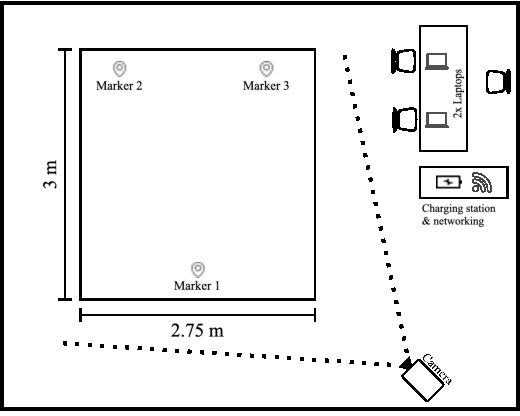
\includegraphics[width=\textwidth]{assets/05/room-layout.pdf}
        \caption{Experimental room layout showing the 3m x 2.75m playspace, researcher station, and equipment placement.}
        \label{fig:room-layout}
    \end{subfigure}
    \hfill
    \begin{subfigure}[b]{0.48\textwidth}
        \centering
        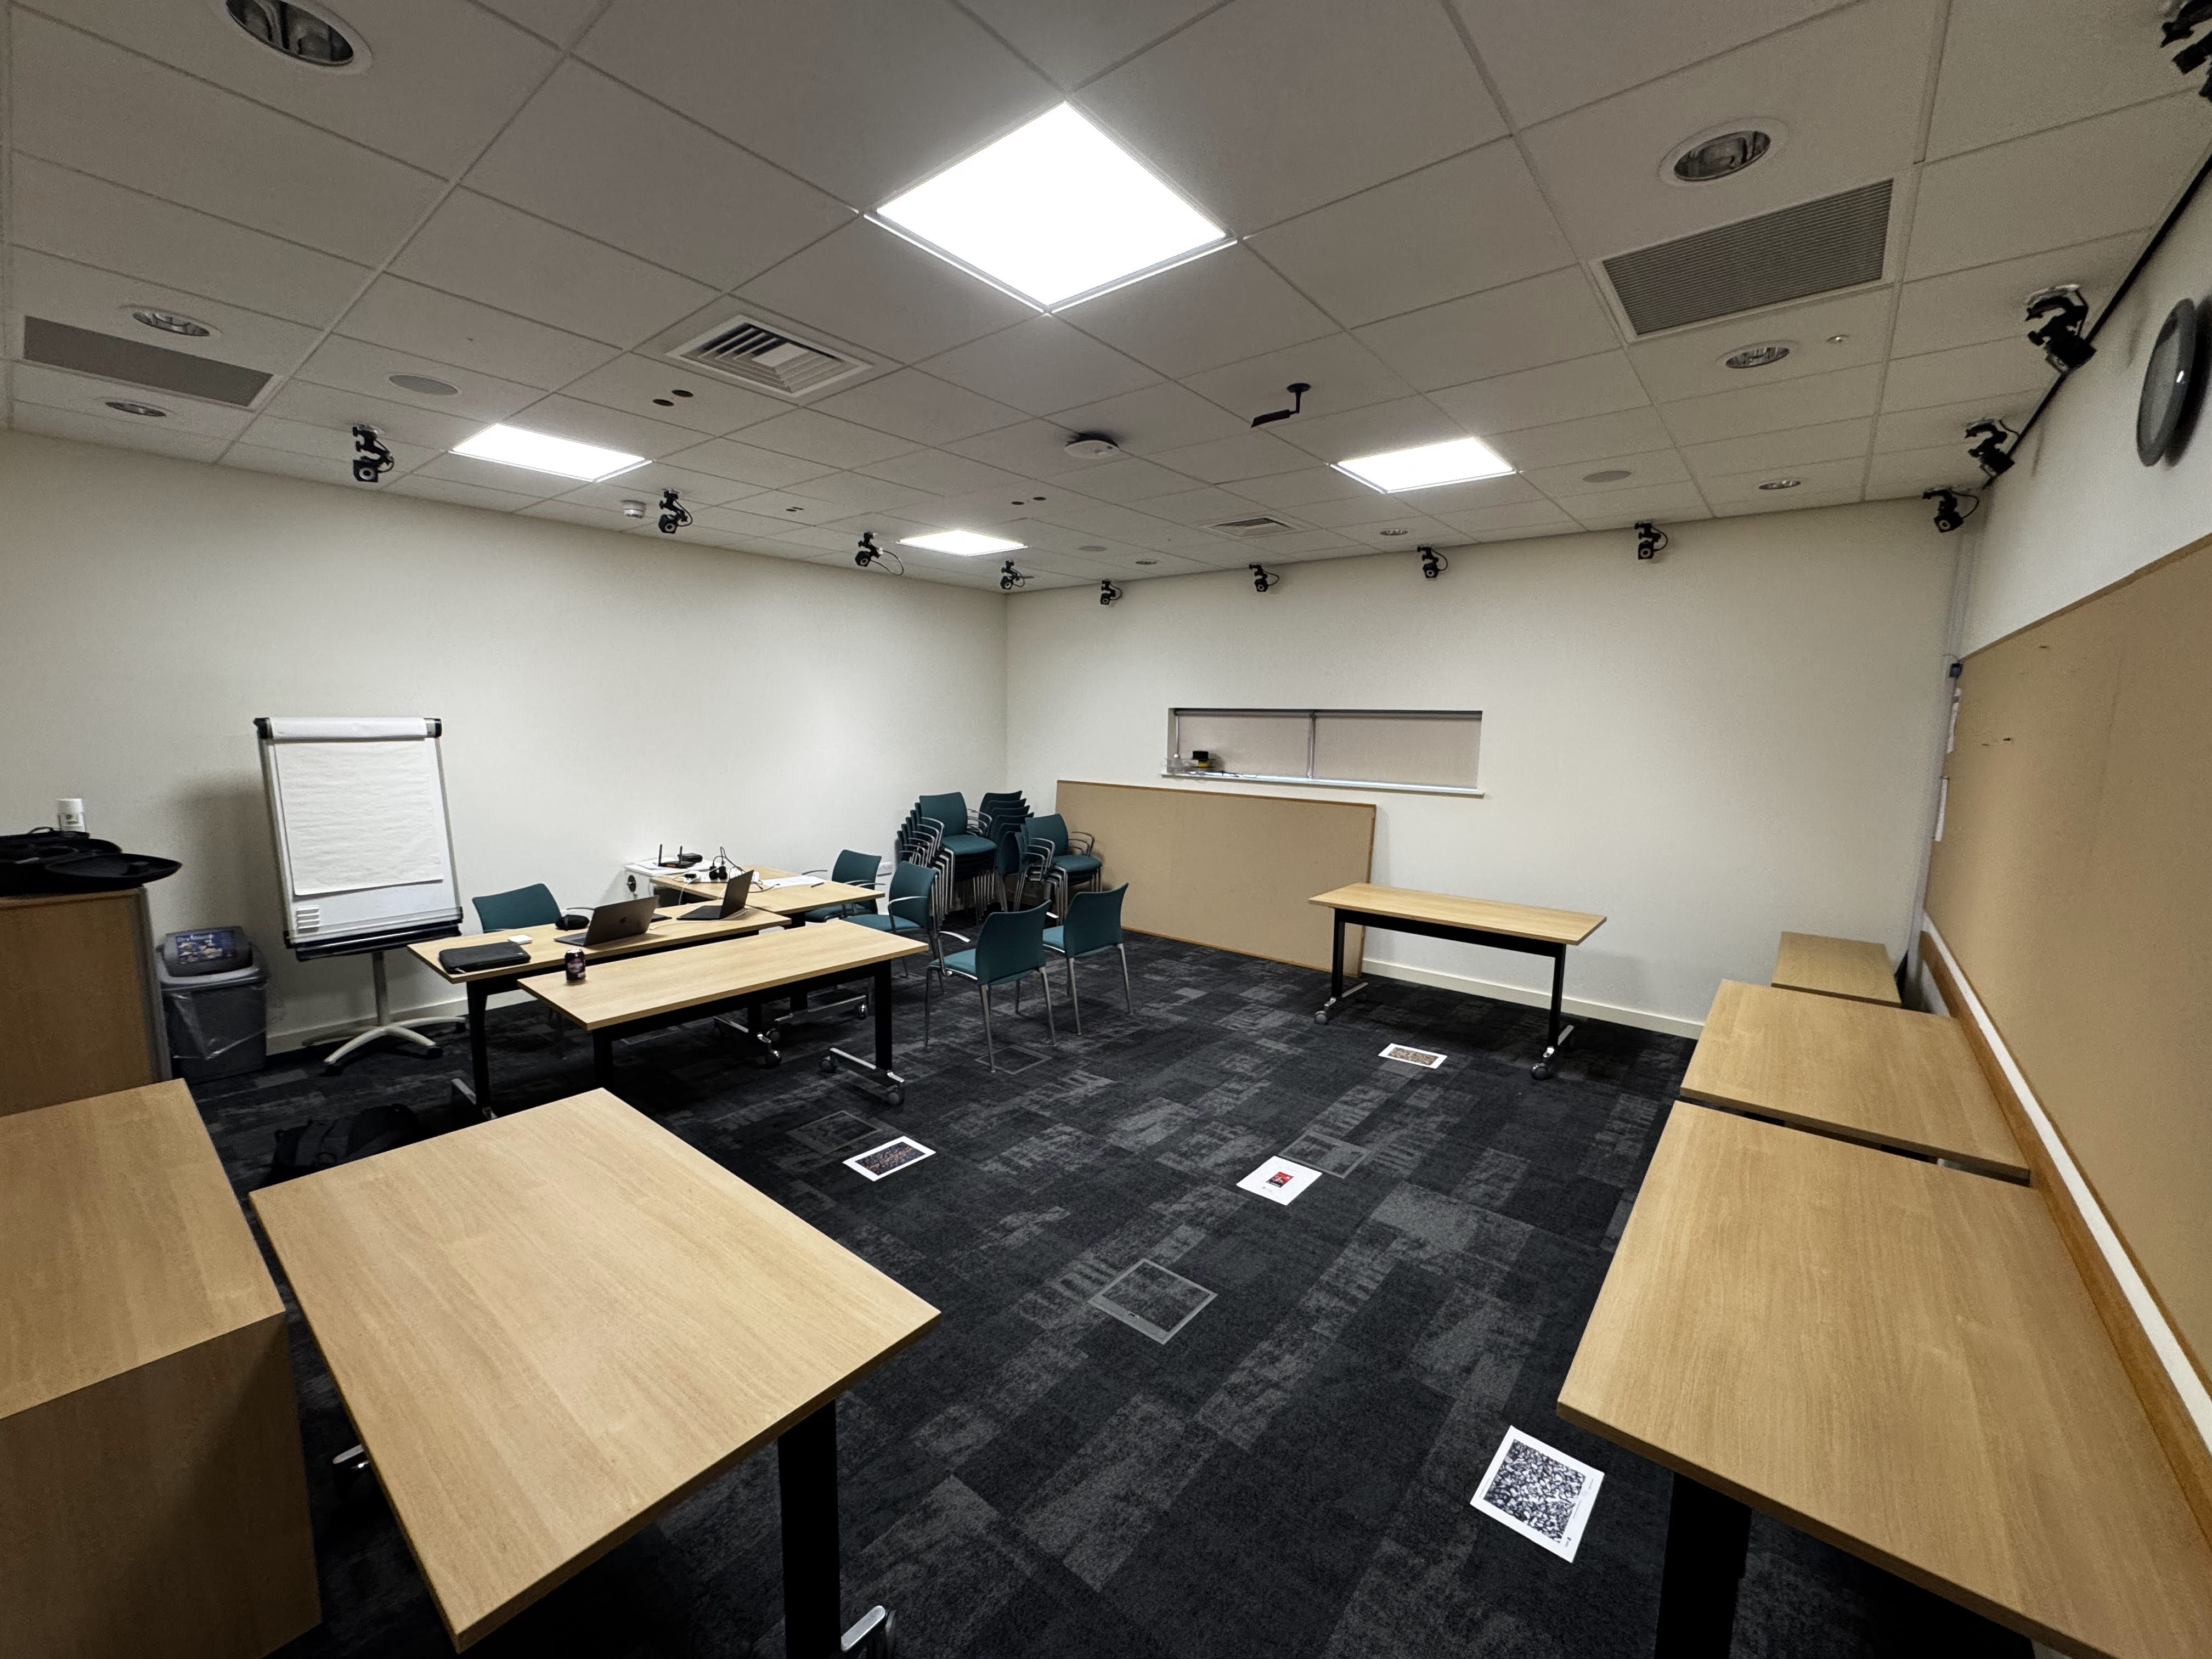
\includegraphics[width=\textwidth]{assets/05/user-study-room.jpg}
        \caption{User study environment showing the room setup with spatial markers on the floor and tables marking the play space.}
        \label{fig:user-study-room}
    \end{subfigure}
    \caption{Experimental environment setup}
    \label{fig:experimental-environment}
\end{figure}

\section{Data Collection}\label{sec:data-collection}

\subsection{Mixed Methods Approach Justification}\label{subsec:mixed-methods-justification}
This study employs a mixed methods approach, combining quantitative measurements (performance metrics, standardised questionnaires) with qualitative data collection (interviews, discussions). Quantitative measures enable statistical analysis and hypothesis testing, while qualitative data captures the nuanced processes underlying collaboration strategies, adaptation mechanisms, and subjective experiences that drive collaborative success or failure. This triangulation approach is particularly suited for exploratory research in human-computer interaction, where complex interactions between technology, task demands, and human factors require both measurement precision and interpretive depth.

Below, all collected metrics, data collection instruments and their respective collection procedures are listed in detail. The full questionnaires as well as interview and discussion protocols are provided in Appendix~\ref{appendix:questionnaires}.

\subsection{Participant Onboarding}\label{subsec:participant-onboarding}
Besides the informed consent (info sheet + presentation), the participants were given a demographic questionnaire to collect information about their background and experience with AR/VR. These variables were recorded to characterise the sample and later examined as potential covariates in the analysis.

\subsection{Questionnaires}\label{subsec:questionnaires}
\subsubsection{Big 5}\label{subsec:big5}
As part of the research question for the user study focussed on the influence of personality on collaboration dynamics, the participants were asked to complete the full 50-item Big 5 personality test \cite{goldberg1992development}. The Big 5 is a widely used personality test that measures the five personality traits: openness to experience, conscientiousness, extraversion, agreeableness, and neuroticism. It exhibits high internal consistency (Cronbach's $\alpha$ = 0.75--0.90) and robust convergent validity with other trait measures\cite{husain2025reliability}. The Big 5 was collected once, before the start of the study.

\subsubsection{NASA TLX}\label{subsec:nasa_tlx}
The NASA Task Load Index (NASA-TLX) \cite{hart1988development} was used to measure the participants' workload and perceived workload during the task. The NASA-TLX is a subjective workload assessment tool that measures the six dimensions of mental, physical, and temporal demand, performance, effort, and frustration of a task on 20-point scales. It exhibits excellent test-retest reliability (r > .80) and sensitivity across human-computer interaction domains\cite{hart1988development, rubio2004evaluation}. The NASA-TLX was collected a total of four times, i.e. after each task variant.

\subsubsection{System Usability Scale}\label{subsec:su}
The System Usability Scale (SUS) \cite{brooke1996sus} was used to measure the participants' perceived ease of use of the AR system. The SUS is a 10-point Likert scale that measures the perceived ease of use of a system. The SUS demonstrates strong reliability (Cronbach's $\alpha$ $\geq$ 0.90) and benchmark data exist for interpreting scores relative to industry standards \cite{bangor2009determining}. The SUS was collected a total of four times, i.e. after each task variant.

\subsubsection{Inclusion of Other in the Self (IOS) Scale}\label{subsec:ios}
To capture perceived interpersonal closeness, we used the pictorial Inclusion of Other in the Self Scale (IOS) \cite{aron1991close}. Participants selected one of seven Venn-diagram pairs ranging from “No overlap” to “Almost complete overlap.” The IOS score shows excellent convergent validity with comprehensive relationship inventories (Spearman's $\rho$ $\approx$ 0.85), while remaining maximally brief \cite{gachter2015measuring}. The IOS was collected twice - once before the study and once after.

\subsubsection{Perceived Competence Scale}\label{subsec:perceived_competence}
A minimally modified variant of the Perceived Competence Scale (PCS) \cite{williams1998perceived} was used to measure the participants' perceived competence after the task. Participants completed this 4-item questionnaire twice per iteration: first rating their own perceived competence, then rating their partner's perceived competence during the collaborative task. There were two iterations of the PCS, once before the study and once after.

\subsubsection{Dyadic Trust Scale}\label{subsec:dyadic_trust}
Trust in one's partner was assessed with the 8-item Dyadic Trust Scale (DTS) \cite{larzelere1980dyadic}. Items are rated on a 7-point Likert scale. The DTS demonstrates strong internal consistency (Cronbach's $\alpha$ $\geq$ 0.89)\cite{larzelere1980dyadic, ccetinkaya2008validity}. The DTS was also collected twice - once before the study and once after.

\subsection{Interviews}\label{subsec:interviews}
\subsubsection{Individual, semi-structured interview}\label{subsec:individual-semi-structured-interview}
Following the completion of all four task variants, each participant underwent an individual semi-structured interview lasting approximately 10-15 minutes. These interviews were conducted separately to ensure candid feedback without partner influence. The interview protocol explored five key dimensions: general experience, task performance, collaboration dynamics, personality influences, and cognitive load.

The interviews began with broad questions about the overall experience, such as "Can you briefly share your overall experience with the task today?" and "Were there moments you particularly enjoyed or felt frustrated?" Participants identified which task variant stood out most prominently and explained their reasoning.

The performance section examined participants' self-assessment of their contributions and evaluation of their partner's performance. This dual perspective revealed potential discrepancies between self-perception and partner perception. The collaboration section probed communication patterns, asking participants to reflect on whether their communication style varied across task variants and how they adapted to different conditions.

Given the study's focus on personality influences, participants reflected on whether their personality traits or previous experience influenced their collaborative approach. This meta-cognitive reflection surfaced participants' theories about their collaborative behaviour, which could be triangulated with Big Five personality scores and observed behaviours. The final section addressed cognitive load, asking participants to identify moments of mental overload and compare relative difficulty across conditions, providing subjective validation of NASA-TLX measurements.

\subsubsection{Semi-structured discussion}\label{subsec:semi-structured-interview}
After both individual interviews were completed, each participant pair engaged in a joint semi-structured discussion lasting approximately 5 minutes. This format captured the collaborative sense-making process, allowing participants to build upon each other's responses and reveal aspects of their shared experience that might not emerge in individual reflection. It also served to observe any difference in answers compared to the individual interviews.

The discussion opened with a warm-up question to establish a comfortable conversational tone: "So, overall—how was that for you two? Anything surprising or memorable?" This encouraged participants to co-construct their narrative of the experience, revealing which aspects they deemed most significant as a pair.

The central focus explored collaboration and communication dynamics through questions requiring participants to reflect on their shared experience: "Did you feel you were on the same page during the building task?" and "Was there a moment when you really clicked, or when you had trouble getting through to each other?" These questions surfaced the participants' joint understanding of their collaborative process, including moments of successful coordination as well as communication breakdowns.

The discussion also examined problem-solving style and contribution patterns, exploring who took initiative during different phases and how responsibilities were distributed. This was particularly valuable for understanding the emergence of leadership roles and task division strategies. The discussion concluded with a forward-looking question: "If you were going to build another bridge together tomorrow, what's one thing you'd want to do differently?" This encouraged participants to synthesize their experience into actionable insights.

\subsection{Instrumented Data Collection}\label{subsec:instrumented-data-collection}
To evaluate the performance of the participants, the following data was collected automatically
\begin{itemize}
    \item \textbf{Video recordings}\label{subsec:video-recordings}, recorded using a separate camera (Apple iPhone 15 Pro Max), position as indicated in Figure~\ref{fig:experimental-environment}.
    \item \textbf{Event logs}\label{subsec:event-logs}, indicating participant positions (at a 1 Hz frequency) and actions (e.g. spawning a block, placing a block, etc.)
    \item \textbf{Screen recordings}\label{subsec:screen-recordings} of the laptop screen, showing the AR system and the participant's actions in real-time.
\end{itemize}

\subsection{Evaluation Metrics}\label{subsec:evaluation-metrics}
Apart from the directly collected data, the following metrics were derived afterwards to evaluate the performance of the participants:
\begin{itemize}
    \item \textbf{Task completion time}\label{subsec:task-completion-time}, measured from the spawn of the first block to the completion of the task.
    \item \textbf{Bridge quality metrics}\label{subsec:bridge-quality}, measured by through the bridge simulations outlined in Chapter~\ref{chapter:artifact-implementation}.
    \item \textbf{Transcripts}\label{subsec:transcripts}, of interactions during each task variant.
\end{itemize}
